\documentclass{../kin_math}

\header{Elijah Kin}{Homework 12}{AMSC660}
\headrule

\begin{document}
The goals of this homework are $(i)$ to acquire practice with real data and $(ii)$ to explore various optimization methods for solving classification problems and understand how their performance is affected by their settings.

\textbf{What to submit.} Please submit a report with figures and comments. Link your codes to the report pdf. These can be e.g. Dropbox links or GitHub links, etc. All optimizers should be coded from scratch.

\textbf{Programming language.} You can use Matlab or Python.
\begin{itemize}
  \item If you are using Matlab, you use MNIST data saved in \texttt{mnist.mat} and my codes \texttt{mnist\_2categories\_quadratic\_NLLS.m} and \texttt{LevenbergMarquardt.m} to get started.
  \item If you are using Python, you use MNIST data saved in \texttt{mnist2.mat} and my codes \texttt{mnist\_2categories\_quadratic\_NLLS.ipynb} and \texttt{LevenbergMarquardt.py} to get started.
\end{itemize}
\section{MNIST dataset}
You will experiment with the MNIST dataset of handwritten digits 0, 1, \dots, 9 available at \url{http://yann.lecun.com/exdb/mnist/}. The training set has 60000 28 x 28 grayscale images of handwritten digits (10 classes) and a testing set has 10000 images. I removed the 4-pixel paddings with zero from these images, making them 20-by-20, with the aid of the code \texttt{readMNIST.m} written by \href{https://www.mathworks.com/matlabcentral/fileexchange/27675-read-digits-and-labels-from-mnist-database}{Siddharth Hegde}.
\section{Classification problem}
The task is to select all images with digits 1 and all images with digits 7 from the training set, find a dividing surface that separates them, and test this dividing surface on the 1's and 7's from the test set. A sample of 1's and 7's from the training set is shown in Fig. 1.
\begin{figure}
  \centering
  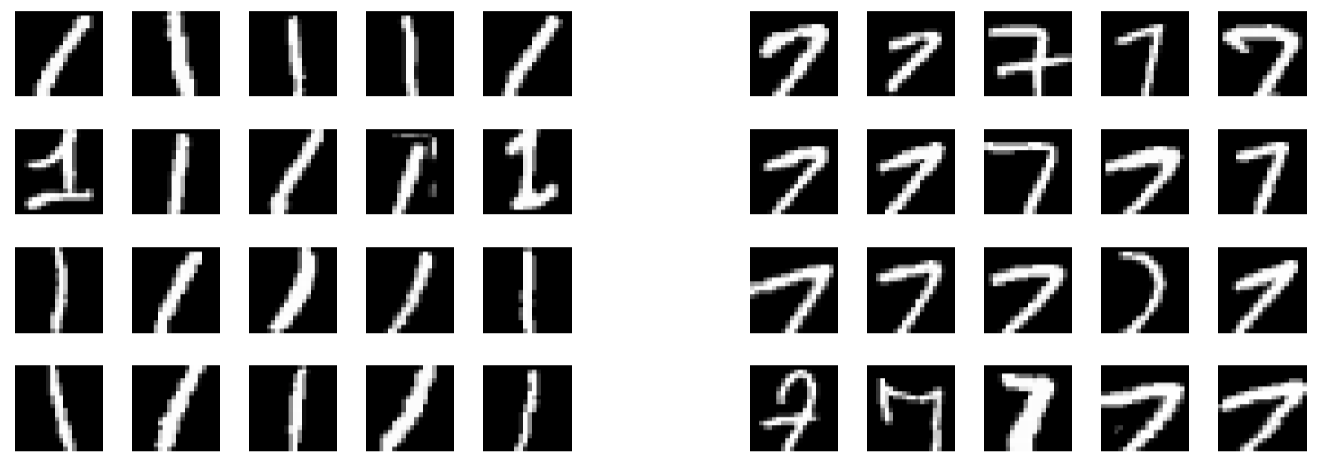
\includegraphics[scale=0.5]{mnist.png}
  \caption{Samples of 20-by-20 images of 1's (left) and 7's (right) from MNIST.}
\end{figure}
Each image is a point in $\mathbb{R}^{400}$ (the images with stripped paddings are 20-by-20). It is convenient to reduce the dimensionality of data by using SVD and mapping the set to $\mathbb{R}^d$ where $d \ll 400$, e.g. $d = 3$, $d = 10$, $d = 20$, etc.

We pose three kinds of unconstrained optimization problems.
\subsection{A smooth loss function for the optimal hyperplane with Tikhonov regularization}
In the simplest setting, we aim at finding a dividing hyperplane $w^\top x + b = 0$ with that $w^\top x_j + b > 0$ for all (almost all) $x_j$ corresponding to 1 (labelled with $y_j = 1$) and $w^\top x_j + b < 0$ for all (almost all) $x_j$ corresponding to 7 (labelled with $y_j = -1$). Hence, $x_j$ is classified
correctly if
\begin{equation*}
  \textsf{sign}(y_j(w^\top x_j + b)) = 1.
\end{equation*}
Instead of the discontinuous \textsf{sign} function, we use a smooth sigmoid-type function (we call it \emph{residual})
\begin{equation}
  r_j \equiv r(x_j; \{w, b\}) \coloneqq \log\left(1 + e^{-y_j(w^\top x_j + b)}\right)
\end{equation}
that is close to zero if $y_j(w^\top x_j + b) > 0$ and grows linearly in the negative range of the aggregate $y_j(w^\top x_j + b)$. For brevity, we will denote the $d + 1$-dimensional vector of parameter $\{w, b\}$ by \textbf{w}. We form the loss function by averaging up the residuals and adding a Tikhonov regularization term:
\begin{equation}
  f(\textbf{w}) = \frac{1}{n} \sum_{j = 1}^n \log\left(1 + e^{-y_j(w^\top x_j + b)}\right) + \frac{\lambda}{2} \lVert \textbf{w} \rVert^2.
\end{equation}
Here $n$ is the number of data points, and $\lambda$ is a parameter for the Tikhonov regularization. $\lambda$ should be a small number. Its purpose is to prevent the entries of $w$ from being too large.
\subsection{A smooth loss function for the optimal quadratic hypersurface with Tikhonov regularization}
As you will see, a quadratic dividing hypersurface may lead to much fewer misclassified digits. We are seeking a quadratic hypersurface of the form:
\begin{equation*}
  x^\top W x + v^\top x + b.
\end{equation*}
Hence, the quadratic test function is
\begin{equation}
  q(x_j; \textbf{w}) \coloneqq y_j(x^\top W x + v^\top x + b).
\end{equation}
The loss function is defined in a similar manner:
\begin{equation}
  \label{eq:loss}
  f(\textbf{w}) = \frac{1}{n} \sum_{j = 1}^n \log\left(1 + e^{-q(x_j; \textbf{w})}\right) + \frac{\lambda}{2} \lVert \textbf{w} \rVert^2.
\end{equation}
Here \textbf{w} denotes the $d^2 + d + 1$-dimensional vector of coefficients of $\{W, v, b\}$.
\subsection{A nonlinear least squares problem for the optimal quadratic hypersurface} \label{least_squares}
Finally, we can design the loss function to fit the framework of the nonlinear least squares problem:
\begin{equation}
  f(\textbf{w}) = \frac{1}{2} \sum_{j = 1}^n [r_j(\textbf{w})]^2, \quad r_j(\textbf{w}) = \log\left(1 + e^{-q(x_j; \textbf{w})}\right).
\end{equation}
The provided codes solve this nonlinear least squares problem and find a dividing quadratic hypersurface using the Levenberg-Marquardt algorithm.
\section{Tasks}
\subsection{Task 1}
Experiment with \textbf{the number of PCAs} using the provided codes. Find out how the number of PCAs affects the number of misclassified digits. Plot a graph of the number of misclassified digits in the test set vs the number of PCAs.
\begin{solution}
  We plot below the number of misclassified digits with each number of PCAs in $\{5, 10, 15, 20, 25\}$. As expected, we find that as the number of PCAs increases, the number of misclassified digits decreases.
  \begin{figure}
    \centering
    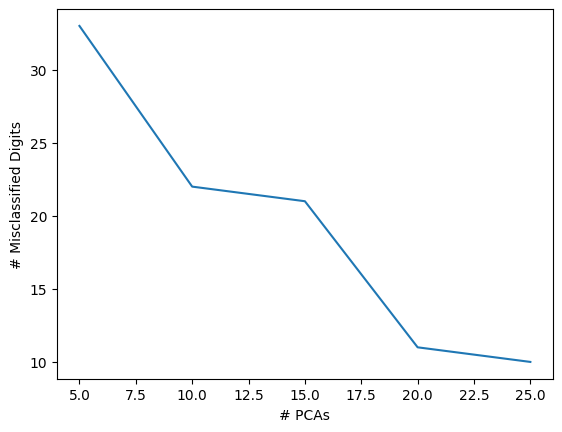
\includegraphics[scale=0.8]{pca.png}
  \end{figure}
\end{solution}
\subsection{Task 2}
Set the number of PCAs to 20. Program the \textbf{Gauss-Newton} algorithm and solve the nonlinear least squares problem in Section \ref{least_squares} using your routine. Plot the graphs of the loss and the norm of the gradient versus iteration number. To avoid problems with inverting the matrix $J^\top J$, you can regularize it by changing it to
\begin{equation*}
  J^\top J + I \cdot 10^{-6}.
\end{equation*}
\begin{solution}
  We implement the Gauss-Newton algorithm \href{https://github.com/elijahkin/amsc660/blob/main/hw12/hw12.ipynb}{here}. With a tolerance of $10^{-3}$, we find that the algorithm misclassifies 20 iterations digits in the test set. We plot the loss and the norm of the gradient of the loss below.
  \begin{figure}
    \centering
    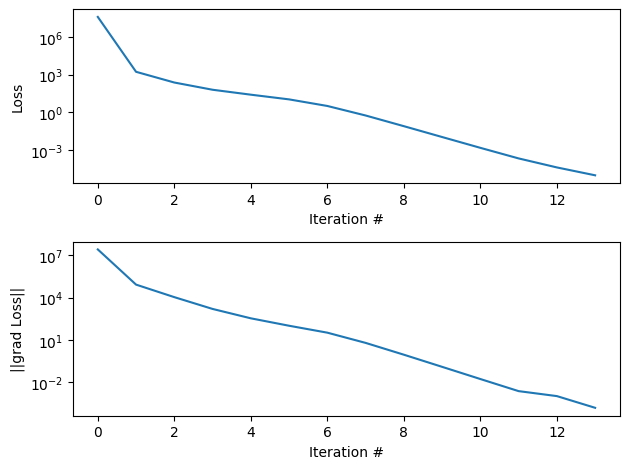
\includegraphics[scale=0.8]{gauss_newton.png}
  \end{figure}
\end{solution}
\subsection{Task 3}
Define the loss function as in (\ref{eq:loss}). Implement \textbf{Stochastic Gradient Descent}. Experiment with various batch sizes and step sizes. Also, try a few stepsize decreasing strategies. Plot the graphs of the loss and the norm of the gradient versus iteration number. Write a summary of your observations. Conclude which batch sizes are reasonable, which stepsizes are reasonable, and how many epochs are enough. Is it beneficial for this problem to use a decreasing step size?
\begin{solution}
  Trying several different values of batch size, step size, and $\lambda$ in the Tikhonov regularization, we find that the best performance occurs with batch size 10, constant $\alpha = 10^{-3}$, and $\lambda = 10^{-4}$, after 100 epochs we misclassify only 11 digits.

  Somewhat counterintuitively, we were unable to best this performance using a decreasing step size, although a decreasing step size should in theory yield better results. We plot the loss and the norm of the gradient of the loss below.
  \begin{figure}
    \centering
    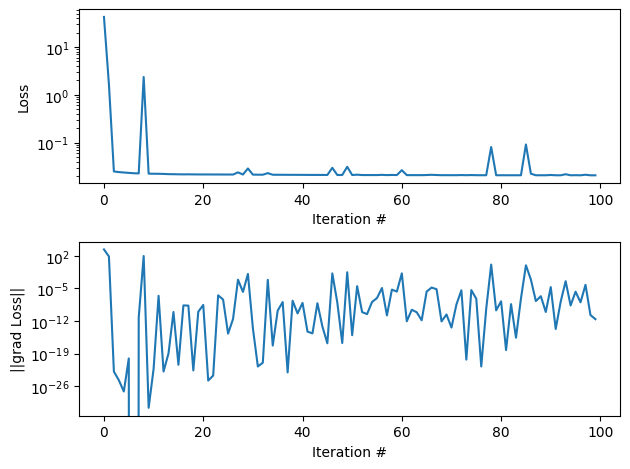
\includegraphics[scale=0.8]{sgd.png}
  \end{figure}
\end{solution}
\end{document}
